% METODOLOGIA------------------------------------------------------------------

\chapter{CRONOGRAMA}
\label{chap:cronograma}
Neste capítulo serão detalhadas as atividades que devem ser executadas até a conclusão deste trabalho, assim como os períodos planejados para a respectiva execução destas.

As tarefas planejadas são a coleta e análise de dados, a fim de verificar a necessidade de adicionar novos tipos de restrições e parametrizações ao otimizador; a execução dos incrementos do software conforme exposto na seção \ref{sec:metodo} e a etapa de validação. Os períodos planejados para cada uma destas atividades constam na \autoref{fig:cronograma}:

\begin{figure}[!htb]
	\centering
	\caption{Cronograma}
	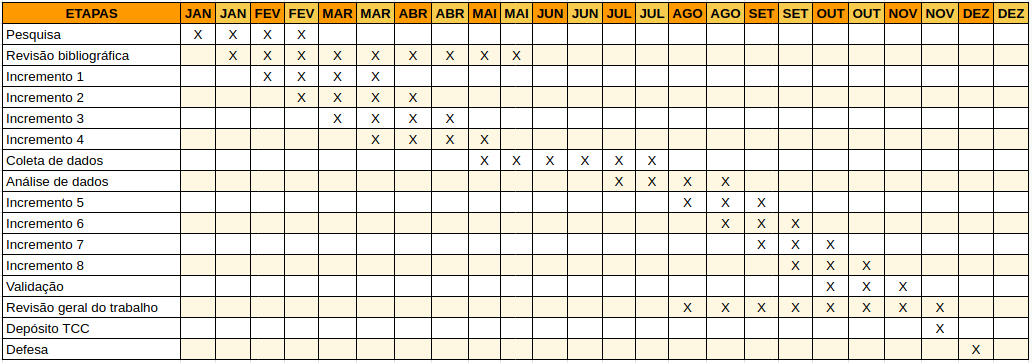
\includegraphics[width=1\textwidth]{./dados/figuras/cronograma}
	\fonte{Autor}
	\label{fig:cronograma}
\end{figure}
